\subsection{The LTCC Window}

The LTCC windows that covers the upstream and downstream open frame of the box is a composite of tedlar/mylar/tedlar, see \F{windowDesign}. The tedlar
material provides light tightness, while the mylar adds the necessary material strength necessary to withstand the gas pressure.

\begin{figure}
	\centering
	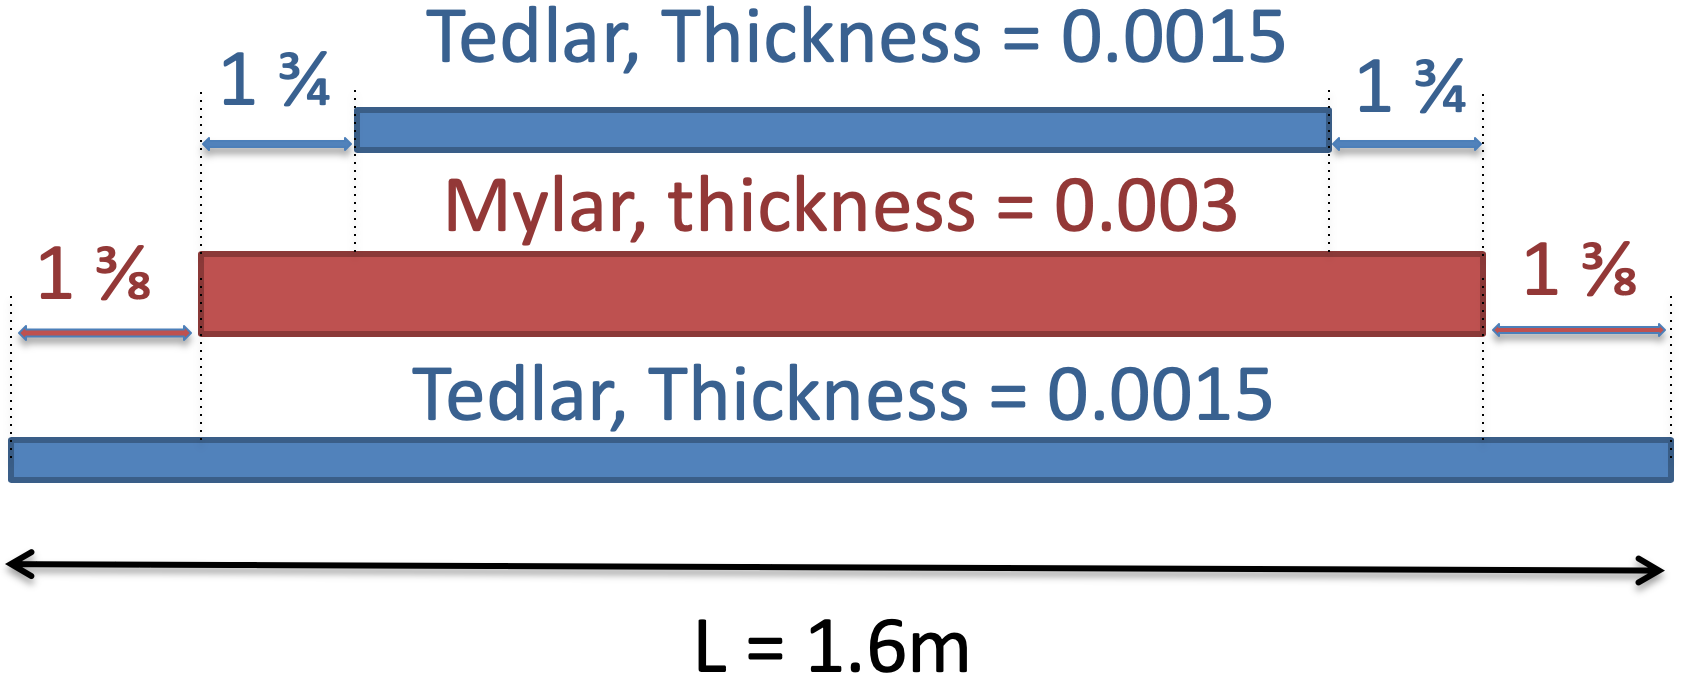
\includegraphics[width=1.0\columnwidth,keepaspectratio]{img/windowDesign.png}
	
\includegraphics[width=1.0\columnwidth,keepaspectratio]{img/windowSeaming.png}
\caption{Top: the design of the window tedlar/mylar/tedlar sandwich. ML is 1.6m. The pyramid design allowed for the seaming shown at the bottom.
			Bottom: the seaming design involves gluing mylar to mylar to ensure that the window stress is transmitted entirely to the mylar. }
	\label{fig:windowDesign}
\end{figure}


The window was fabricated in two steps:

\begin{enumerate}
	\item lamination of tedlar/mylar/tedlar rolls 1.6m  wide
	\item seaming of the laminated strips into 4.8mx4.8m window
\end{enumerate}

The lamination of 400 yards of the composite material has been performed at Madico \cite{madico}.

\subsubsection{Windows seaming and tests}

The 1.6 m wide windows are seamed together using GLUE USED? The seam has been load tested to withstand a pressure test 10 times
higher than the expected pressure from the gas flow and gas weight, see \F{windowTest}.


\begin{figure}
	\centering
	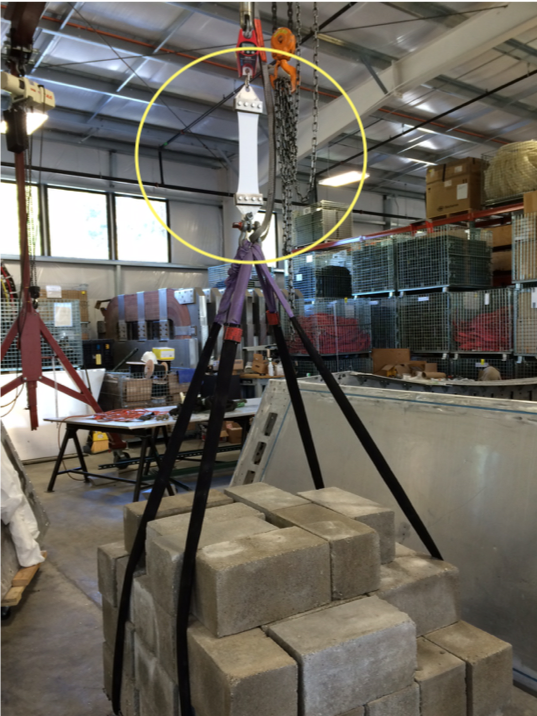
\includegraphics[width=1.0\columnwidth,keepaspectratio]{img/windowTest.png}
	\caption{The window was tested with up to 388 lbs of load. No significant damage was observed until rupture, which occured at a load of 388 lbs,
			   corresponding to about 15,000 psi of stress on the window, about a factor of 10 higher than the stress during normal operations of the detector.}
	\label{fig:windowTest}
\end{figure}

\subsubsection{Windows installation and gas leaks tests}

The installation of the window onto the box is achieved through glueing the window on the box sides. GLUE USED? METHOD DETAILS.
An example of the downstream window after installation is shown in \F{downstreamWindow}.

\begin{figure}
	\centering
	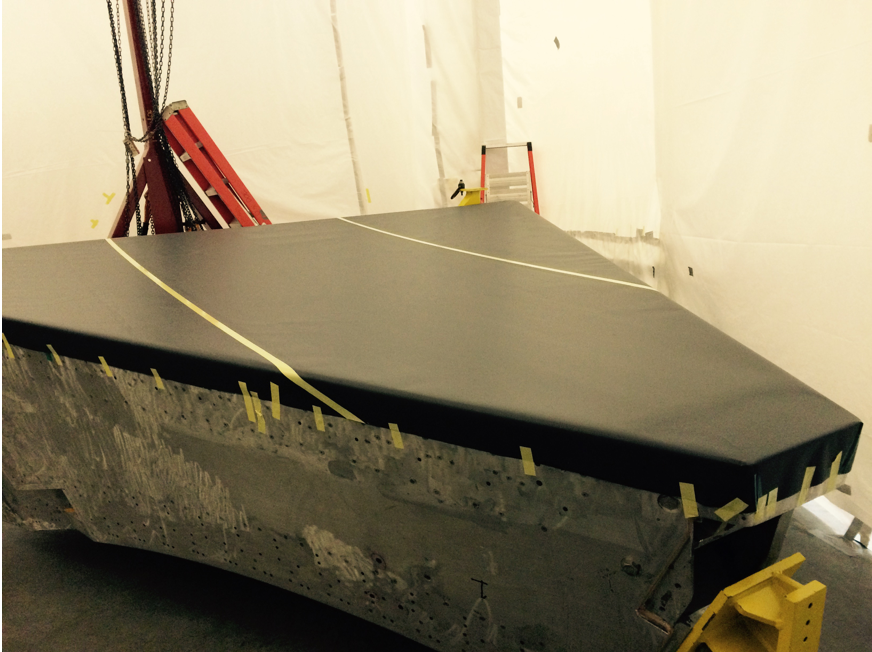
\includegraphics[width=1.0\columnwidth,keepaspectratio]{img/downstreamWindow.png}
	\caption{The downstream window of one LTCC sectors during curing of the glue. }
	\label{fig:downstreamWindow}
\end{figure}

After curing of both upstream and downstream window, the LTCC box is filled with nitrogen gas to a pressure of 2 inches of water.
Freon gas is pumped in the box and leaks are detected using a refrigerant leak detector. After the leaks are stopped, the box is pressurized
for a 48 hour period to test the frame overall gas tightness. This procedure was repeated after every movement of the LTCC boxes, as small
shifts of the frame walls introduced additional leaks.

